

Cztery cechy węzłów poznane w poprzednim rozdziale: liczba gordyjska, mostowa i patykowa oraz indeks skrzyżowaniowy są dla nas kompletnie bezużyteczne.
Ich użyteczność dla nas jest ograniczona, bo nie widać wcale, jak wyznaczyć wartość którejkolwiek z~nich.
Dlatego teraz wprowadzimy 3-kolorowania z którym nie dość, że będziemy odróżniać pewne węzły od niewęzła, to jeszcze odróżnimy te węzły od siebie!

Splot nazywamy 3-kolorowalnym, jeżeli jego włókna dają się pokolorować trzema barwami tak, by nie złamać magicznych reguł (które podamy).
Nie potrzeba przewidującej przyszłość kuli, żeby wpaść na pomysł rozszerzenia palety do większej liczby barw.
Dalej uogólniać można na dwa sposoby: albo zastępujac kolory elementami nieprzemiennej grupy (i dostać etykietowania), albo zamiast zliczać kolorowania zbadać relacje między nimi.
Wstęp nie jest miejscem na tłumaczenie detali, więc wspomnimy krótko, że grupy $\Z/p\Z \oplus \Z/p\Z$ oraz $\Z/p^2 \Z$ są równoliczne, ale nie izomorficzne, bo tylko jedna z nich jest cykliczna.

Ani kolorowanie, ani etykietowanie nie są zupełne: to znaczy istnieją węzły, których nie potrafią od siebie odróżnić.
Wszystkie niezmienniki poza całką Koncewicza na pewno mają tę wadę.
Całka Koncewicza (opisana w sekcji \ref{sec:vassiliev}) być może też jest wadliwa.
Nie wiadomo.

\section{Kolorowanie splotów}
\index{kolorowalność|(}%

Przygodę z kolorowaniami rozpoczyna się zazwyczaj od trójkolorowalności.
Jest to pewna cecha diagramów, którą można posiadać albo nie.

\begin{definition}[trójkolorowalność]
\index{trójkolorowalność}%
    Niech $D$ będzie diagramem splotu $L$, którego łuki występują w~trzech kolorach.
    Jeżeli spełnione są następujące warunki:
    \begin{itemize}[leftmargin=*]
        \item nie wszystkie łuki są tego samego koloru,
        \item przy każdym skrzyżowaniu spotykają się albo trzy łuki w trzech różnych kolorach, albo wszystkie tego samego koloru,
    \end{itemize}
    to mówimy, że diagram $D$ jest trójkolorowalny.
\end{definition}

Splot posiadający trójkolorowalny diagram nazywamy krótko trójkolorowalnym.
Często można spotkać się też z trójkolorowalność Foxa, szczególnie w anglojęzycznych materiałach, ale my nie czujemy potrzeby używania długiej nazwy.

\begin{examplenosquare}
    Lorem ipsum dolor sit amet, consectetur adipiscing elit. Donec hendrerit felis nec sollicitudin scelerisque. Etiam odio urna, faucibus eget sodales a, sollicitudin ut odio. Interdum et malesuada fames ac ante ipsum primis in faucibus. Sed metus urna, vehicula eu efficitur quis, interdum pellentesque tellus. Vestibulum ex neque, sagittis nec hendrerit a,~eleifend vitae ligula. Donec ut erat erat.
    \begin{figure}[H]
        \begin{minipage}[b]{.14\linewidth}
            {\hfill\color{white}.}
        \end{minipage}
        \begin{minipage}[b]{.35\linewidth}
            \centering
            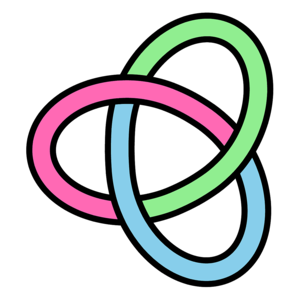
\includegraphics[height=2.2cm]{../data/fox-coloring/3_1.png}
            \subcaption{trójlistnik jest 3-kolorowalny,}
        \end{minipage}
        \begin{minipage}[b]{.35\linewidth}
            \centering
            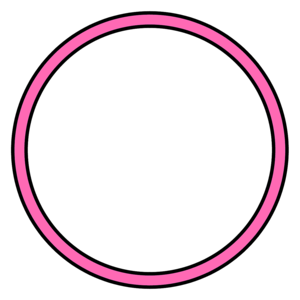
\includegraphics[height=2.2cm]{../data/knots/0_1.png}
            \subcaption{niewęzeł nie jest 3-kolorowalny.}
        \end{minipage}
        \begin{minipage}[b]{.14\linewidth}
            \hfill {\tiny\ensuremath{\blacksquare}}
        \end{minipage}
    \end{figure}
\end{examplenosquare}

Tak naprawdę pokazaliśmy tylko, że niewęzeł ma niekolorowalny diagram, ale czy nie może on mieć innego diagramu, który jest kolorowalny?
Nie może, co wynika bezpośrednio z~faktu \ref{prp:colouring_invariance}.

Dla wygody jako kolorów używać będziemy kolejnych liczb naturalnych $0, 1, \ldots, n-1$
(przez ostatnią stronę mieliśmy $n = 3$).
Pozwala to zapisać warunek ,,być kolorowalnym'' równaniem algebraicznym, niezależnie od ilości użytych kolorów.

\begin{definition}[kolorowanie]
\index{równanie kolorujące}%
\label{def:colouring_equation}%
    Niech $L$ będzie splotem, zaś $n$ liczbą naturalną.
    Mówimy, że splot $L$ jest kolorowalny modulo $n$, jeśli posiada diagram, którego włóknom można przypisać liczby całkowite $0, \ldots, n - 1$ tak, by
    \begin{enumerate}
        \item istniały dwa włókna różnych kolorów,
        \item równanie $a + b \equiv 2c$ modulo $n$ było spełnione przy każdym skrzyżowaniu:
    \end{enumerate}
\begin{comment}
    \[
        \LargePlusCrossingColouring
    \]
\end{comment}
    Takie przyporządkowanie nazywamy kolorowaniem.
\end{definition}

Nie potrafimy ustalić, kto pierwszy napisał jawnie równanie ,,$a + b \equiv 2c$ modulo $n$'' myśląc o~kolorowaniach.
Być może był to Ralph Fox, który około 1956 roku chciał uczynić teorię węzłów bardziej przystępną dla studentów koledżu Haverford w Pensylwanii; on jednak nie pisał ,,trójkolorowalne węzły'', tylko ,,węzły z własnością L''.
(Znaczenia litery L także nie potrafimy ustalić).
Ale nie wolno zapominać, że już Reidemeister rozpatrywał reprezentacje grupy węzła $\pi$ na grupę diedralną $D_{2n}$.

\begin{proposition}
\label{prp:colouring_invariance}%
    Własność ,,być $n$-kolorowalnym'' jest niezmiennikiem węzłów.
\end{proposition}

\begin{proof}
    Po przypisaniu kolorów górnym włóknom widzimy, że kolory wszystkich pozostałych włókien są wymuszone przez równanie kolorujące przy kolejnych skrzyżowaniach.
    Dlatego sprawdzimy, że wykonanie dowolnego ruchu Reidemeistera nie psuje kolorowalności reszty diagramu.
    
    Zacznijmy od ruchu pierwszego i~drugiego:
\begin{comment}
    \begin{figure}[H]
    \centering
    %
    \begin{minipage}[b]{.4\linewidth}
        \[
            \LargeReidemeisterOneLeftProof \stackrel{R_1}{\cong} \LargeReidemeisterOneStraightProof
        \]
    \end{minipage}
    %
    \begin{minipage}[b]{.5\linewidth}
        \[
            \LargeReidemeisterTwoColouringA \stackrel{R_2}{\cong} \LargeReidemeisterTwoColouringB
        \]
    \end{minipage}
    \end{figure}
\end{comment}
    Trzeci ruch także nie wymaga skomplikowanych rachunków.
    Najkrótszy łuk na diagramach ma kolor $2a-c$ po lewej oraz $2b-c$ po prawej stronie.
\begin{comment}
    \[
        \LargeReidemeisterThreeColouringA \cong \LargeReidemeisterThreeColouringB
    \]
\end{comment}
    Ponownie wykonianie ruchu Reidemeistera nie zmienia kolorów dolnych włókien.
\end{proof}

Trójlistnik koloruje się dokładnie modulo krotności trójki, ósemka zaś -- piątki.
Sama kolorowalność nie mówi wiele, splot jest kolorowalny lub nie.
Dowód faktu \ref{prp:colouring_invariance} pokazuje coś więcej: liczba kolorowań, być może trywialnych (czyli takich, gdzie użyto tylko jednego koloru), jest mocniejszym niezmiennikiem.

\begin{lemma}
\label{lem:colouring_arc}%
    Ustalmy diagram $D$ dla węzła z~wybranym łukiem, oraz kolor $k \in \{0, \ldots, n - 1\}$.
    Bez straty ogólności możemy założyć, że krótki łuk jest koloru $k$.
\end{lemma}

Kolorem tym zazwyczaj jest $0$.

\begin{proof}
    Dodanie tej samej wartości do wszystkich łuków na dobrze pokolorowanym diagramie daje nowy, także dobrze pokolorowany diagram.
\end{proof}

\begin{proposition}
\label{prp:no_colourings_mod_2}%
    Żaden węzeł nie koloruje się modulo dwa.
\end{proposition}

\begin{proof}
    Załóżmy nie wprost, że istnieje nietrywialne kolorowanie.
    Analiza czterech możliwych skrzyżowań pokazuje, że włókna wychodzące z~tunelu muszą mieć ten sam kolor.
    Przechodząc wzdłuż węzła widzimy jeden kolor, wbrew założeniu nie wprost.
\end{proof}

\begin{proposition}
\label{prp:links_colouring_like_a_lot}%
    Każdy splot o co najmniej dwóch ogniwach koloruje się modula dwa.
\end{proposition}

\begin{proof}
    Wystarczy pomalować jedną składową zerem, a~pozostałe jedynkami.
\end{proof}

Sploty rozszczepialne są $n$-kolorowalne dla każdego $n \ge 2$, można skorzystać z~tego samego schematu kolorowania.
\index{splot!rozszczepialny}%
Pierścienie Boromeuszy nie kolorują się modulo trzy, nie są zatem rozszczepialne.
\label{boromean_not_splittable}%
\index{pierścienie Boromeuszy}%

Sploty, które nie są kolorowalne modulo $n$ dla żadnej liczby $n \in \N$ nazywa się czasem niewidzialnymi, tę własność mają dwa węzły pierwsze o dziesięciu skrzyżowaniach ($10_{124}$, $10_{153}$), cztery o jedenastu ($11n_{34}$, $11n_{42}$, $11n_{49}$, $11n_{116}$) oraz jedenaście o dwunastu ($12n_{19}$, $12n_{121}$, $12n_{210}$, $12n_{214}$, $12n_{242}$, $12n_{292}$, $12n_{309}$, $12n_{313}$, $12n_{318}$, $12n_{430}$, $12n_{473}$).
\index{węzeł!niewidzialny}%
% ZWERYFIKOWANO: funkcja invisible_knots

Pokażemy teraz, że suma równań kolorujących z dobrze wybranymi znakami jest postaci $0 \equiv 0 \mod n$.
Jest to składnik w dowodzie na to, że wyznacznik determinuje kolorowalność splotu.
Będziemy potrzebować pomocniczej definicji.

\begin{definition}[uszachowienie]
\index{uszachowienie}%
    Niech $D$ będzie ustalonym diagramem splotu $L$.
    Jego dopełnienie do płaszczyzny składa się z rozłącznych obszarów.
    Pomalowanie niektórych obszarów tak, żeby każda nić leżała na brzegu dokładnie jednego kolorowego obszaru, nazywamy uszachowieniem diagramu $D$.
\end{definition}

Dla oszczędności tuszu w drukarce zazwyczaj zaczyna się od białej płaszczyzny i używa szarego do kolorowania, ale w tej książce wszędzie, gdzie to tylko możliwe, obecny jest różowy i uszachowienia nie będą stanowić wyjątku.

Ustalmy węzeł $K$ oraz dowolne uszachowienie dla jego diagramu.
Skojarzmy z~każdym skrzyżowaniem równanie kolorujące, zgodnie z~poniższym schematem:
\begin{comment}
\begin{figure}[H]
    \begin{minipage}[b]{.48\linewidth}
    \[
        \LargeCrossingChessboardA
    \]
    \subcaption{$+a-b+a-c=0 \mod n$}
    \end{minipage}
    \begin{minipage}[b]{.48\linewidth}
    \[
        \LargeCrossingChessboardB
    \]
    \subcaption{$-a+b-a+c=0 \mod n$}
    \end{minipage}
\end{figure}
\end{comment}

\begin{proposition}
\label{prp:colouring_sum_zero}%
    Sumą równań kolorujących o dobrze wybranych znakach jest $0 \equiv 0 \mod n$.
\end{proposition}

\begin{proof}
    Każde równanie kolorujące składa się z~czterech wyrazów, po jednym od każdej nici, która spotyka się w~danym skrzyżowaniu.
    Nić biegnie między dwoma skrzyżowaniami, więc suma wszystkich równań kolorujących składa się z~par składników, po jednej parze na nić.
    Składniki te są przeciwnych znaków, zatem wzajemnie się znoszą.
    Suma równań kolorujących jest sumą zer, a~to należało udowodnić.
\end{proof}

Liczbę kolorowań splotu $L$ modulo $n$, trywialnych lub nie, oznaczamy przez $\tau_n(L)$.

\begin{proposition}
    Niech $K_1, K_2$ będą węzłami.
    Wtedy 
    \begin{equation}
        \frac{\tau_3(K_1 \shrap K_2)}{3} = \frac{\tau_3(K_1)}{3} \cdot \frac{\tau_3(K_2)}{3}.
    \end{equation}
\end{proposition}

\begin{corollary}
    Istnieje nieskończenie wiele węzłów.
\end{corollary}

\begin{proof}
    Suma spójna $n$ trójlistników ma $3^{n+1}$, trywialnych lub nie, $3$-kolorowań.
\end{proof}

Niskowymiarowa topologia byłaby miałka, gdyby źródłem nieskończoności węzłów była tylko operacja $\shrap$.
O wielu niezmiennikach węzłów złożonych podejrzewamy albo wiemy, że wyrażają się w terminach mniejszych węzłów pierwszych, oprócz wspomnianej tu liczby kolorowań mamy hipotezy \ref{con:crossing_additive}, \ref{conjecture_unknotting_additive}, nienazwane oszacowanie na stronie \pageref{stick_bounded_factors}, fakty \ref{lem:det_multiplicativ}, \ref{prp:alexander_multiplicative}, \ref{prp:homfly_and_shraps}, \ref{prp:genus_of_sum}, \ref{prp:signature_additive}, \ref{cor:arf_adds}.
Na szczęście fakt \ref{prop:infinite_prime_knots_1} głosi, że węzłów pierwszych też jest nieskończenie wiele; po prostu jesteśmy jeszcze za głupi, aby podać jego dowód.

% Koniec sekcji Kolorowanie splotów


\section{Etykietowanie}
%\index{etykietowanie|(}%

Dotychczas kolorowaliśmy diagramy węzłów liczbami $0, 1, 2, \ldots, n-1$, czyli elementami grupy $\Z/n\Z$, ale nic nie stoi na przeszkodzie, żeby próbować użyć dowolnej innej skończonej grupy.
Etykietowalność to niezmiennik, który uogólnia kolorowalność.
Poznaliśmy go dzięki książce Livingstona \cite[s. 89-99]{livingston1993}, ale poza panem Charlesem mało kto o nim wspomina!

\begin{definition}[etykietowanie]
    Niech $G$ będzie skończenie generowaną grupą, zaś $D$ diagramem zorientowanego węzła $K$.
    Surjekcję ze zbioru włókien diagramu $D$ na zbiór generatorów grupy $G$ taką, że przy każdym skrzyżowaniu spełnione jest równanie $g_Ug_L = g_Rg_U$ (z oznaczeniami jak na rysunku: włókno $g_U$ biegnie górą; włókna $g_L$, $g_R$ po lewej i prawej stronie podskrzyżowania), nazywamy etykietowaniem diagramu $D$ grupą $G$.
    Węzeł, który posiada diagram etykietowalny grupą $G$ też nazywamy etykietowalnym grupą $G$.
\begin{comment}
        \[
            \LargePlusCrossingLabel
        \]
\end{comment}
\end{definition}

Równanie $g_R = g_Ug_Lg_U^{-1}$ mówi, że etykiety włókien wchodzących oraz wychodzących są sprzężone.
Wynika stąd, że wszystkie etykiety pochodzą z~jednej klasy sprzężoności.
Muszą jednocześnie generować całą grupę, dlatego $G$ musi być grupą nieprzemienną lub trywialną.
Etykietowalność jest niezmiennikiem węzłów i~nie zależy od orientacji węzła: jeżeli elementy $g_1, \ldots, g_n$ generują grupę, to ich odwrotności także.

Etykietowania są naturalnym uogólnieniem kolorowań.
Dlaczego?
% Pokazuję i objaśniam - Małgorzata K.
Niech $p \ge 3$ będzie liczbą pierwszą, natomiast $D_p = \langle r, s \mid r^p = s^2 = e, rsr = s \rangle$ grupą diedralną rzędu $2p$.
Elementy tej grupy to $1, r, r^2, \ldots, r^{p-1}, s, sr, \ldots, sr^{p-1}$.
,,Obrót'' $r^k$ jest sprzężony tylko ze swoją odwrotnością (mamy $sr^lr^k(sr^l)^{-1} = sr^ks = r^{-k}$), ale ,,symetrie osiowe'' $sr^k$ tworzą jedną klasę sprzężoności.
Łatwo widać, że dowolne dwie z~nich generują całą grupę $D_p$.

\begin{proposition}
    Węzeł $K$ jest $p$-kolorowalny wtedy i~tylko wtedy, gdy jest $D_p$-etykietowalny.
\end{proposition}

\begin{proof}
    Załóżmy, że $K$ ma $n$ włókien.
    Wiemy już, że każde $D_p$-etykietowanie wykorzystuje tylko elementy $sr^{a_1}, \ldots, sr^{a_n}$ dla $1 \le a_i \le p$.
    Jest ono prawidłowe dokładnie wtedy, gdy analogiczne kolorowanie liczbami $a_1, \ldots, a_n$ jest prawidłowe.
\end{proof}

Pozostało wskazać parę węzłów, których nie odróżniają kolorowania, ale odróżnia pewne etykietowanie.

\begin{example}
    Węzeł $9_{46}$ jest etykietowalny grupą $S_4$, wystarczy jego włóknom dobrze przypisać transpozycje (niech to będzie proste ćwiczenie dla Czytelnika).
    Węzeł $6_1$ nie jest etykietowalny tą samą grupą.
    Wybranie dwóch etykiet przy jednym skrzyżowaniu wymusza etykiety dla wszystkich włókien, ale dwie grupy nie mogą generować grupy $S_4$.
    Węzły te są więc różne.
\end{example}

Węzły $6_1$ i $9_{46}$ mają ten sam wielomian Alexandera, zatem ten sam wyznacznik, więc na mocy faktu \ref{prp:colour_determinant} te same własności kolorujące.
\index{wielomian Alexandera}%
Dużo później odkryliśmy parę jeszcze raz w~\cite[s. 138]{burde2014}, gdzie pokazano, że  $E_2(6_1) = \Z(t)$; $E_2(9_{46}) = (t-2, 2t-1)$.
Niestety nie wiemy, kto pierwszy wpadł na ten pomysł porównania ich ideałów elementarnych $E_2$. 

Etykietowanie jest mocnym narzędziem odróżniającym węzły.
Thistlethwaite w 1985 roku korzystając z niego klasyfikował węzły o~co najwyżej 13 skrzyżowaniach (jest ich, jak ostatecznie się okazało, 12965).
\index[persons]{Thistlethwaite, Morwen}%
Mają one tylko 5639 różnych wielomianów Alexandera, ale etykietowania trzynastoma różnymi grupami pozwoliły zmniejszyć liczbę nierozpoznanych węzłów do około tysiąca.
Wśród nich 30 posiada wielomian Conwaya $1 + 2z^2 + 2z^4$, ale pary rozróżniane wielomianem HOMFLY mają też różne wielomiany Jonesa.

Kolorowania definiowano kiedyś jako surjekcje $\rho \colon \pi \to D_{2n}$ z~grupy podstawowej.
Jak mówi prezentacja Wirtingera, grupa splotu generowana jest przez ścieżki z~punktu bazowego w~$S^3$ do brzegu rurowego otoczenia splotu, wokół południka i~znowu do bazowego punktu.
\index{prezentacja Wirtingera}%
Fox zauważył, że z~surjektywności $\rho$ wynika, iż generatory mapują się na symetrie osiowe $sr^k$.
Ponieważ istnieje wzajemnie jednoznaczna odpowiedniość między generatorami grupy splotu oraz łukami diagramu, każdemu możemy przypisać liczbę całkowitą $k$.
Etykietowania są więc uogólnieniem kolorowań.
Rozumowanie, które przedstawiliśmy, prowadzi do prostej klasyfikacji grup, których można użyć do etykietowania.

\begin{proposition}
    Niech $K$ będzie węzłem, $\pi$ grupą podstawową jego dopełnienia, zaś $G$ dowolną grupą.
    Następujące warunki są równoważne: $K$ jest $G$-etykietowalny; istnieje surjekcja $\pi_1 \to G$.
\end{proposition}

Historycznie, prezentacja Wirtingera była pierwsza, zaś etykietowania odkryto później.
% TODO: ustalić, kiedy później

\begin{proposition}[Perko]
    Niech $K$ będzie węzłem.
    Następujące warunki są równoważne: $K$ jest etykietowalny grupą $S_3$, $K$ jest etykietowalny grupą $S_4$.
\end{proposition}
% To jest w https://faculty.etsu.edu/gardnerr/Knot-Theory/Notes-Livingston/Livingston-Knot-5-2.pdf, ale nie książce Livingston a livingston1993

\begin{proof}
    Dowód zajmuje tylko kilka stron i składa się z dwóch części.
    Po pierwsze $S_4$ ma podgrupę czwórkową Kleina, więc istnieje epimorfizm $S_4 \to S_3$; pozwala to opuszczać epimorfizmy $G \to S_4$ do epimorfizmów $G \to S_3$.
    
    Jak podnosić epimorfizmy $G \to S_3$ do epimorfizmów $G \to S_4$ pokazał Perko \cite{perko1975}.
\end{proof}

Nie znamy innych nietrywialnych faktów dotyczących etykietowań.

\index{etykietowanie|)}%



\index{kolorowalność|)}%

